\chapter{Data Experiments}
\label{ch5}
In this chapter, the parts that compose this project as well as their context are shown. Also, some experiments are demonstrated for comparison with different parameters that could affect this thesis' project's overall accuracy.

\section{Inputs and Outputs}
In previous chapters, it has been specified that this algorithm takes an text input and, according to its contents, a message is shown as an output. The breakdown is as follows.
\subsection{Inputs}
The input that is given is cleaned up and tokenized -- as shown in \nameref{ch4} --, this is then added to an internal corpus that has weights set for every word in it, effectively working as scores. Every word has a different score in every label, whether it is positive or negative. This score is added up and the highest final score will be the one that the algorithm will detect as the most probable for the text input. However, this has its caveats, small sentences are more likely to be miscategorized because one word can have different applications in the scope of this project, for a more accurate analysis a longer sentence must be written.
\subsection{Outputs}
Depending on the final score, the algorithm will choose a random sentence related to the detected sentiment, this is, as of the time of writing, very rudimentary, but the fact that it is built in Python this can be a building block for a more robust, context-conscious, reply system.
In the training module, however, four extra values are part of the output as well: \texttt{Loss}, \texttt{Val\_loss}, \texttt{Accuracy} and \texttt{Val\_accuracy}.
These values are standard in every Neural Network algorithm to observe how poorly the evaluation does within the training dataset, and what the accuracy percentage is, respectively.
The \texttt{Val\_} counterparts of these values are the same, but applied to the validation dataset.

\section{Experiments}
In this section, various experiments of this project are shown with varying training data and parameters with the respective accuracy and loss graphs.
The purpose of these experiments is to determine if the parameters chosen for this project are optimal and, if not, correct them and know the reason behind the improvement.
The parameters that could potentially have a great impact on the output of the classification -- and therefore are the best to experiment with -- are the following:
\begin{itemize}
	\item Used datasets: This could influentiate the amount of words in the corpus and have a big impact on how some words are percieved
	\item Training epochs: How many loops does the algorithm go through before being considered fully trained, if this number is too high it could result in \textit{overfitting}, which is, in casual terms, the Neural Network equivalent of overthinking.
	\item Units in the LSTM layer: This unit system, albeit small in the overall scale of things, could make-or-break the algorithm if not tuned correctly.
	\item Categorized sentiments: Reducing the scope of the project could potentially benefit the overall accuracy of the remaining sentiments.
\end{itemize}
The amount of improvement with each experiment is shown with loss and accuracy graphs, which are evaluated every epoch the algorithm is trained. Lower loss and higher accuracy are preferred.
\subsection{Experiment 1: Base Experiment}
\label{exp1}
In this experiment, we look at the base version of this thesis' project.
\begin{table}[!th]
	\caption{Experiment 1's defining characteristics.}
	\vspace{0.5cm}
	\centering
	\begin{tabular}[t]{|l|l|}
	\hline
		Datasets Used & 2: \citet{d1} and \citet{d2}
	\\ \hline
		Epochs & 10
	\\ \hline
		LSTM Layer & 32 units
	\\ \hline
		Categorized Sentiments as ``Bad'' & ``Sadness'', ``Worry'', and ``Fear''.
	\\ \hline	
		 Categorized Sentiments as ``Neutral'' & ``Neutral'' and ``Boredom''.
	\\ \hline	
		Categorized Sentiments as ``Good'' & ``Happiness'', ``Fun'', ``Joy'', and ``Love''.
	\\ \hline
	\end{tabular}
\end{table}

\begin{figure}[!h]
	\centering
	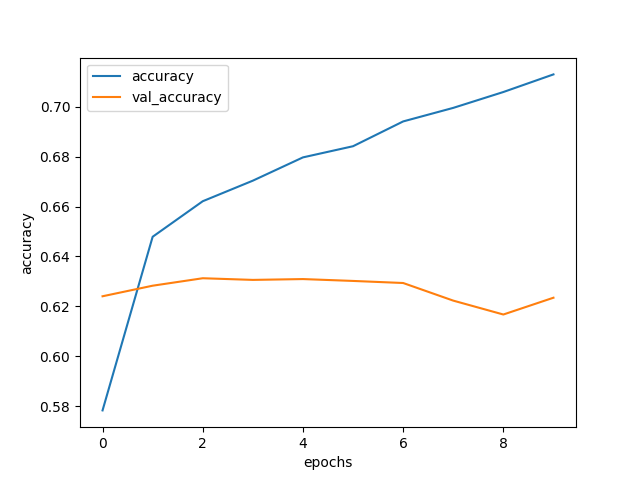
\includegraphics[scale=0.8]{Accuracy_Exp1}
	\caption{Accuracy Graph of Experiment 1}
	\label{fig:accuracy_exp1}
	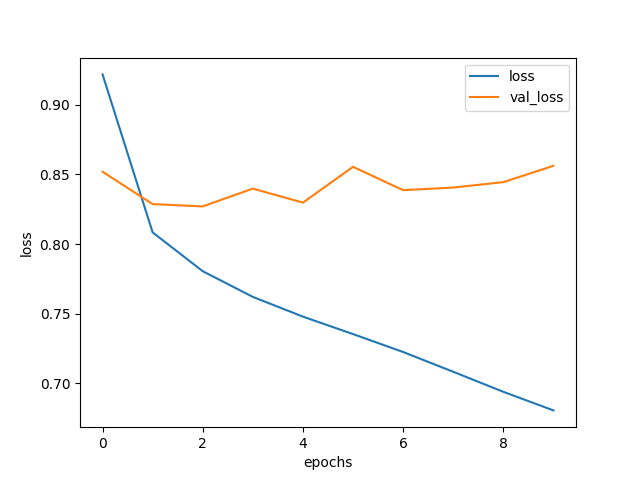
\includegraphics[scale=0.8]{Loss_Exp1}
	\caption{Loss Graph of Experiment 1}
	\label{fig:loss_exp1}
\end{figure}
\pagebreak

\subsection{Experiment 2: More Datasets With Reduced Data Scope}
\label{exp2}
This experiment takes sentences from one more dataset and 3 less categorized sentiments: ``Fear'', ``Joy'', and ``Love''.
\begin{table}[!th]
	\caption{Experiment 2's defining characteristics.}
	\vspace{0.5cm}
	\centering
	\begin{tabular}[t]{|l|l|}
	\hline
		Datasets Used & \makecell{3: \citet{d1}, \citet{d2} and\\ \citet{d3}}
	\\ \hline
		Epochs & 10
	\\ \hline
		LSTM Layer & 32 units
	\\ \hline
		Categorized Sentiments as ``Bad'' & ``Sadness'', and ``Worry''.
	\\ \hline	
		 Categorized Sentiments as ``Neutral'' & ``Neutral'' and ``Boredom''.
	\\ \hline	
		Categorized Sentiments as ``Good'' & ``Happiness'', and ``Fun''.
	\\ \hline
	\end{tabular}
\end{table}

\begin{figure}[!h]
	\centering
	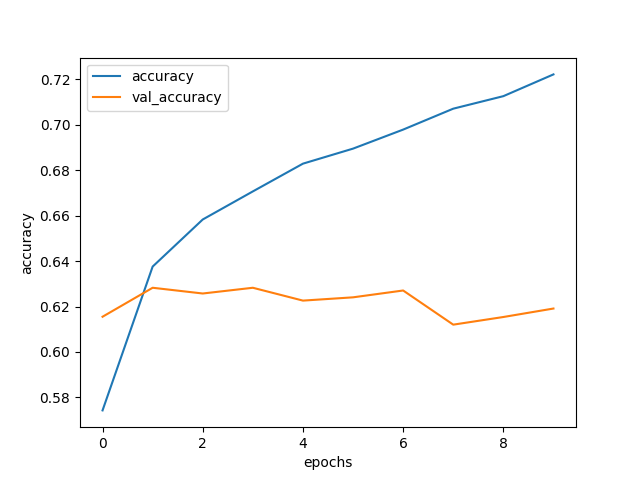
\includegraphics[scale=0.8]{Accuracy_Exp2}
	\caption{Accuracy Graph of Experiment 2}
	\label{fig:accuracy_exp2}
	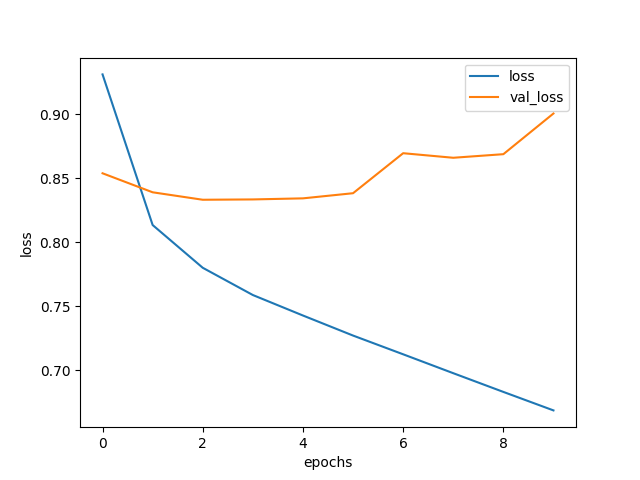
\includegraphics[scale=0.8]{Loss_Exp2}
	\caption{Loss Graph of Experiment 2}
	\label{fig:loss_exp2}
\end{figure}
\pagebreak

\subsection{Experiment 3: Augmented LSTM Units}
\label{exp3}
Largely the same as Experiment 2, but the LSTM has more units to work with.
\begin{table}[!th]
	\caption{Experiment 3's defining characteristics.}
	\vspace{0.5cm}
	\centering
	\begin{tabular}[t]{|l|l|}
	\hline
		Datasets Used & \makecell{3: \citet{d1}, \citet{d2} and\\ \citet{d3}}
	\\ \hline
		Epochs & 10
	\\ \hline
		LSTM Layer & 64 units
	\\ \hline
		Categorized Sentiments as ``Bad'' & ``Sadness'', and ``Worry''.
	\\ \hline	
		 Categorized Sentiments as ``Neutral'' & ``Neutral'' and ``Boredom''.
	\\ \hline	
		Categorized Sentiments as ``Good'' & ``Happiness'', and ``Fun''.
	\\ \hline
	\end{tabular}
\end{table}

\begin{figure}[!h]
	\centering
	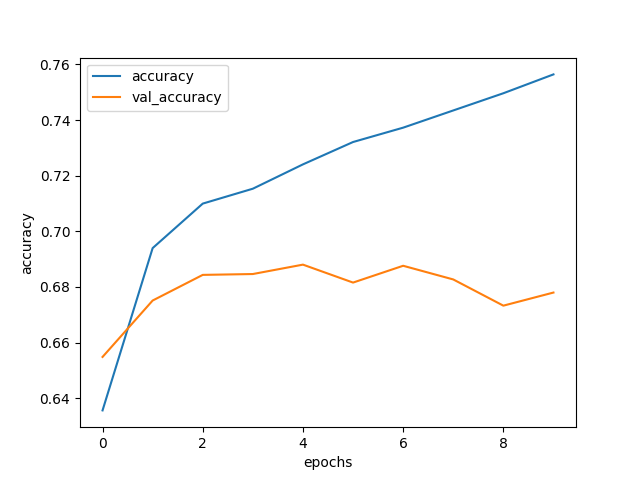
\includegraphics[scale=0.8]{Accuracy_Exp3}
	\caption{Accuracy Graph of Experiment 3}
	\label{fig:accuracy_exp3}
	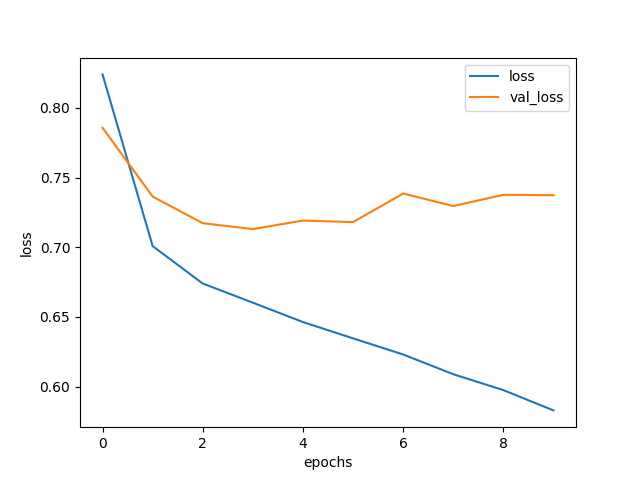
\includegraphics[scale=0.8]{Loss_Exp3}
	\caption{Loss Graph of Experiment 3}
	\label{fig:loss_exp3}
\end{figure}
\pagebreak

\subsection{Experiment 4: Augmented Datasets Without Reduced Data Scope}
\label{exp4}
A mix between Experiment 1 and 2. Three datasets with the full sentiment categorization and LSTM with 32 units.
\begin{table}[!h]
	\caption{Experiment 4's defining characteristics.}
	\vspace{0.5cm}
	\centering
	\begin{tabular}[t]{|l|l|}
	\hline
		Datasets Used & \makecell{3: \citet{d1}, \citet{d2} and\\ \citet{d3}}
	\\ \hline
		Epochs & 10
	\\ \hline
		LSTM Layer & 32 units
	\\ \hline
		Categorized Sentiments as ``Bad'' & ``Sadness'', ``Worry'', and ``Fear''.
	\\ \hline	
		 Categorized Sentiments as ``Neutral'' & ``Neutral'' and ``Boredom''.
	\\ \hline	
		Categorized Sentiments as ``Good'' & ``Happiness'', ``Fun'', ``Joy'', and ``Love''.
	\\ \hline
	\end{tabular}
\end{table}

\begin{figure}[!h]
	\centering
	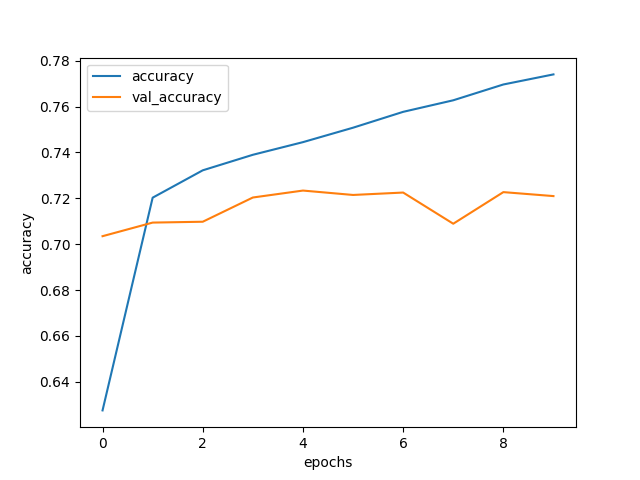
\includegraphics[scale=0.8]{Accuracy_Exp4}
	\caption{Accuracy Graph of Experiment 4}
	\label{fig:accuracy_exp4}
	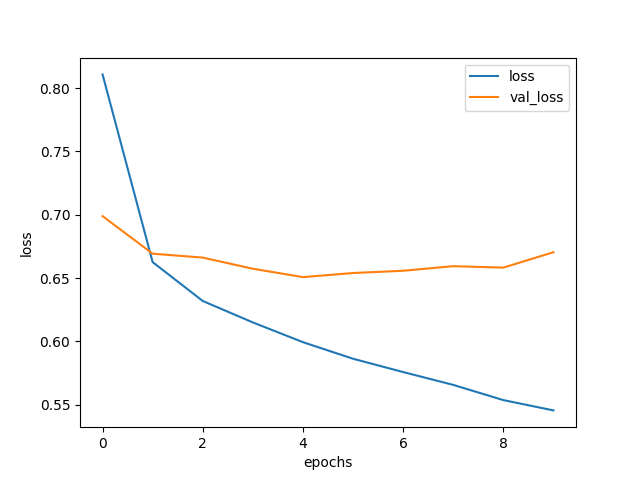
\includegraphics[scale=0.8]{Loss_Exp4}
	\caption{Loss Graph of Experiment 4}
	\label{fig:loss_exp4}
\end{figure}
\pagebreak

\subsection{Experiment 5: Extra Sadness Dataset}
\label{exp5}
Same as Experiment 4, but with an added dataset with only ``Sadness'' sentences.
\begin{table}[!h]
	\caption{Experiment 5's defining characteristics.}
	\vspace{0.5cm}
	\centering
	\begin{tabular}[t]{|l|l|}
	\hline
		Datasets Used & \makecell{4: \citet{d1}, \citet{d2},\\ \citet{d3}, and \citet{d4}}
	\\ \hline
		Epochs & 10
	\\ \hline
		LSTM Layer & 32 units
	\\ \hline
		Categorized Sentiments as ``Bad'' & ``Sadness'', ``Worry'', and ``Fear''.
	\\ \hline	
		 Categorized Sentiments as ``Neutral'' & ``Neutral'' and ``Boredom''.
	\\ \hline	
		Categorized Sentiments as ``Good'' & ``Happiness'', ``Fun'', ``Joy'', and ``Love''.
	\\ \hline
	\end{tabular}
\end{table}

\begin{figure}[!h]
	\centering
	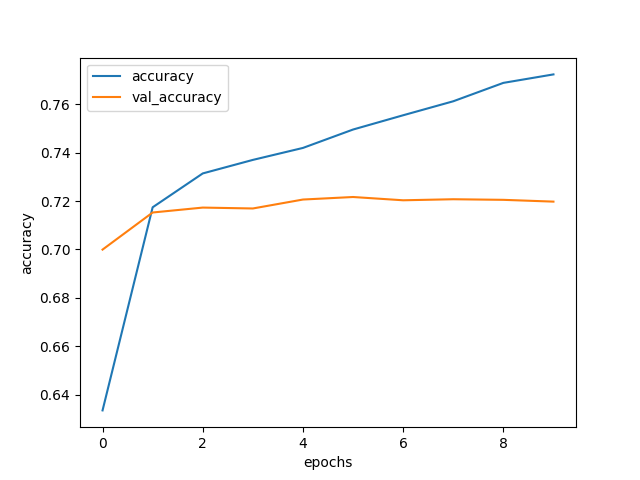
\includegraphics[scale=0.8]{Accuracy_Exp5}
	\caption{Accuracy Graph of Experiment 5}
	\label{fig:accuracy_exp5}
	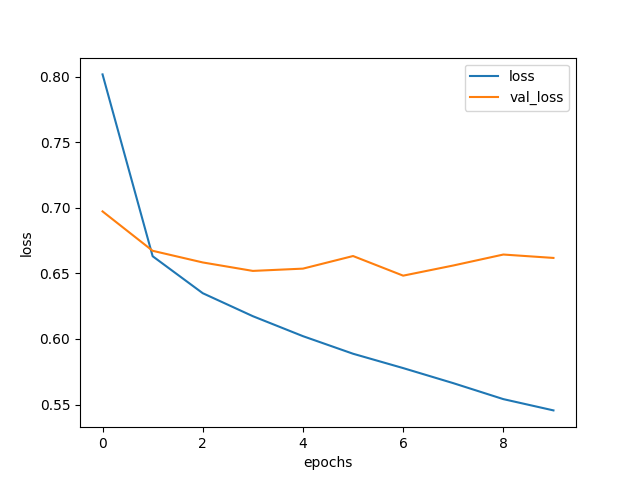
\includegraphics[scale=0.8]{Loss_Exp5}
	\caption{Loss Graph of Experiment 5}
	\label{fig:loss_exp5}
\end{figure}
\pagebreak

\subsection{Experiment 6: Reduced Classification Scope}
\label{exp6}
This is the largest change on an experiment, the ``Neutral'' category has been completely disabled with the purpose of seeing how the rest of the data would be classified as.
\begin{table}[!h]
	\caption{Experiment 6's defining characteristics.}
	\vspace{0.5cm}
	\centering
	\begin{tabular}[t]{|l|l|}
	\hline
		Datasets Used & \makecell{4: \citet{d1}, \citet{d2},\\ \citet{d3}, and \citet{d4}}
	\\ \hline
		Epochs & 10
	\\ \hline
		LSTM Layer & 32 units
	\\ \hline
		Categorized Sentiments as ``Bad'' & ``Sadness'', ``Worry'', and ``Fear''.
	\\ \hline	
		 Categorized Sentiments as ``Neutral'' & N/A
	\\ \hline	
		Categorized Sentiments as ``Good'' & ``Happiness'', ``Fun'', ``Joy'', and ``Love''.
	\\ \hline
	\end{tabular}
\end{table}

\begin{figure}[!h]
	\centering
	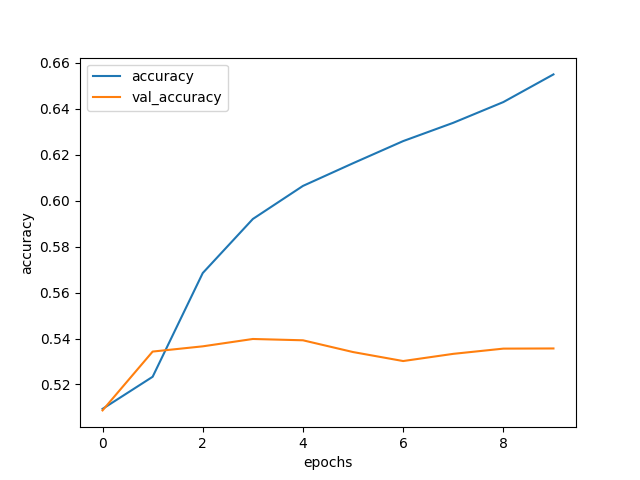
\includegraphics[scale=0.8]{Accuracy_Exp6}
	\caption{Accuracy Graph of Experiment 6}
	\label{fig:accuracy_exp6}
	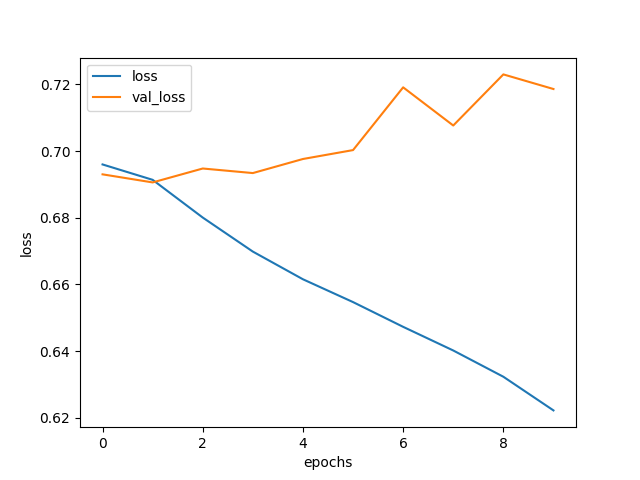
\includegraphics[scale=0.8]{Loss_Exp6}
	\caption{Loss Graph of Experiment 6}
	\label{fig:loss_exp6}
\end{figure}
\pagebreak

\subsection{Experiment 7: Reduced Epochs}
\label{exp7}
Largely the same as Experiment 5 with half the epochs. This with the purpose of seeing if the data has been overfit.
\begin{table}[!h]
	\caption{Experiment 7's defining characteristics.}
	\vspace{0.5cm}
	\centering
	\begin{tabular}[t]{|l|l|}
	\hline
		Datasets Used & \makecell{4: \citet{d1}, \citet{d2},\\ \citet{d3}, and \citet{d4}}
	\\ \hline
		Epochs & 5
	\\ \hline
		LSTM Layer & 32 units
	\\ \hline
		Categorized Sentiments as ``Bad'' & ``Sadness'', ``Worry'', and ``Fear''.
	\\ \hline	
		 Categorized Sentiments as ``Neutral'' & ``Neutral'' and ``Boredom''.
	\\ \hline	
		Categorized Sentiments as ``Good'' & ``Happiness'', ``Fun'', ``Joy'', and ``Love''.
	\\ \hline
	\end{tabular}
\end{table}


\begin{figure}[!h]
	\centering
	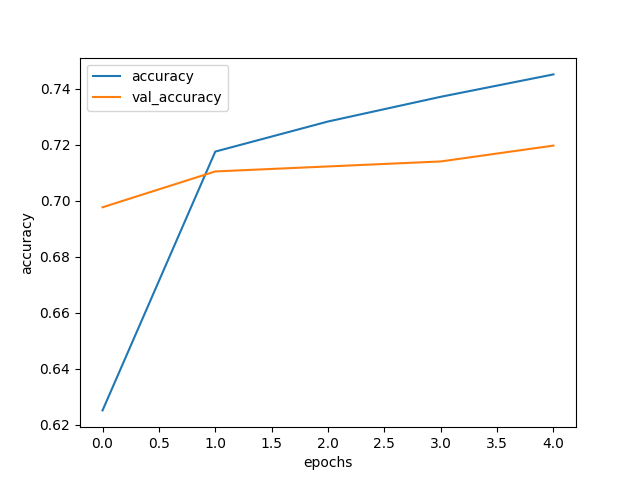
\includegraphics[scale=0.8]{Accuracy_Exp7}
	\caption{Accuracy Graph of Experiment 7}
	\label{fig:accuracy_exp7}
	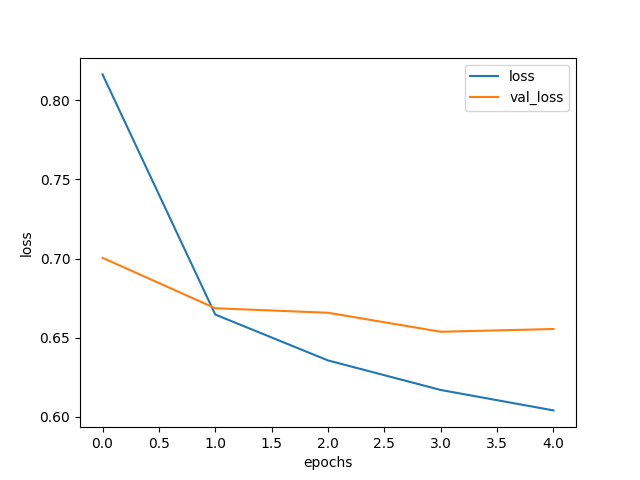
\includegraphics[scale=0.8]{Loss_Exp7}
	\caption{Loss Graph of Experiment 7}
	\label{fig:loss_exp7}
\end{figure}
\pagebreak

\subsection{Experiment 8: Added Stop Words}
\label{exp8}
Same as the experiment 7, the difference being that the top 3 most recurrent words in the datasets are flagged as stop words in an attempt to mitigate the bleed between categories.
\begin{table}[!h]
	\caption{Experiment 8's defining characteristics.}
	\vspace{0.5cm}
	\centering
	\begin{tabular}[t]{|l|l|}
	\hline
		Datasets Used & \makecell{4: \citet{d1}, \citet{d2},\\ \citet{d3}, and \citet{d4}}
	\\ \hline
		Epochs & 5
	\\ \hline
		LSTM Layer & 32 units
	\\ \hline
		Categorized Sentiments as ``Bad'' & ``Sadness'', ``Worry'', and ``Fear''.
	\\ \hline	
		 Categorized Sentiments as ``Neutral'' & ``Neutral'' and ``Boredom''.
	\\ \hline	
		Categorized Sentiments as ``Good'' & ``Happiness'', ``Fun'', ``Joy'', and ``Love''.
	\\ \hline
	\end{tabular}
\end{table}


\begin{figure}[!h]
	\centering
	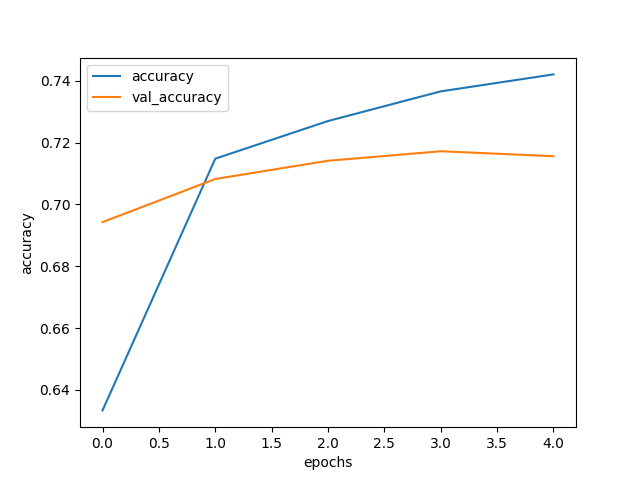
\includegraphics[scale=0.8]{Accuracy_Exp8}
	\caption{Accuracy Graph of Experiment 8}
	\label{fig:accuracy_exp8}
	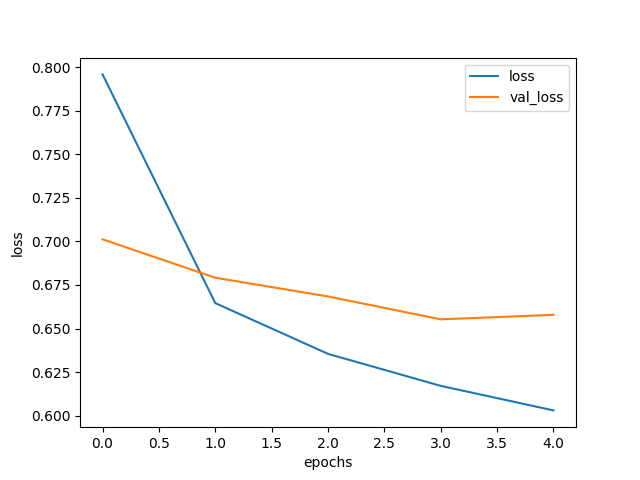
\includegraphics[scale=0.8]{Loss_Exp8}
	\caption{Loss Graph of Experiment 8}
	\label{fig:loss_exp8}
\end{figure}
\pagebreak

\subsection{Experiment 9: Extra Stop Words and Reduced Classification Scope}
\label{exp9}
Keeping in track with experiment 8, with the added extra of also reducing the scope of the classification, reducing the categories to ``Good'' and ``Bad''.
\begin{table}[!h]
	\caption{Experiment 9's defining characteristics.}
	\vspace{0.5cm}
	\centering
	\begin{tabular}[t]{|l|l|}
	\hline
		Datasets Used & \makecell{4: \citet{d1}, \citet{d2},\\ \citet{d3}, and \citet{d4}}
	\\ \hline
		Epochs & 5
	\\ \hline
		LSTM Layer & 32 units
	\\ \hline
		Categorized Sentiments as ``Bad'' & ``Sadness'', ``Worry'', and ``Fear''.
	\\ \hline	
		Categorized Sentiments as ``Good'' & ``Happiness'', ``Fun'', ``Joy'', and ``Love''.
	\\ \hline
	\end{tabular}
\end{table}


\begin{figure}[!h]
	\centering
	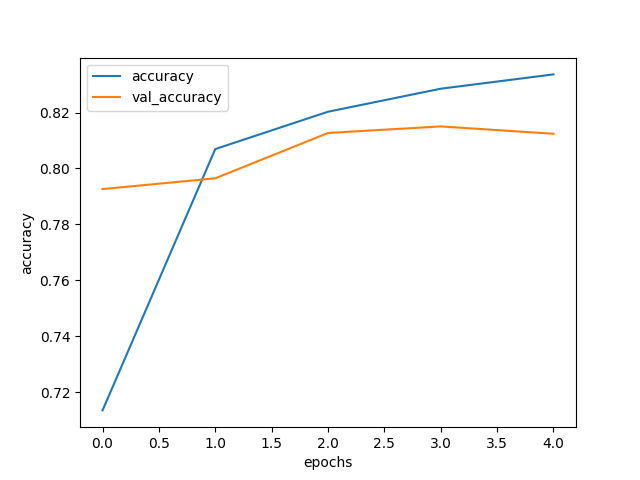
\includegraphics[scale=0.8]{Accuracy_Exp9}
	\caption{Accuracy Graph of Experiment 9}
	\label{fig:accuracy_exp9}
	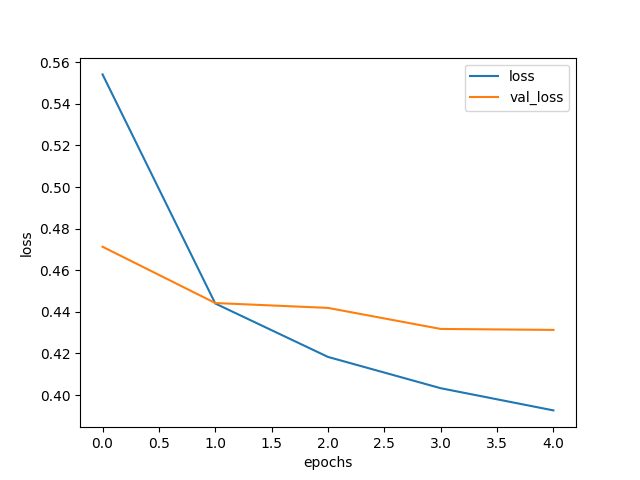
\includegraphics[scale=0.8]{Loss_Exp9}
	\caption{Loss Graph of Experiment 9}
	\label{fig:loss_exp9}
\end{figure}
\pagebreak

\section{Results}
In this section, the results of the experiments from the previous section will be discussed. Later on, a hypothesis will be formulated based from them. For reference, all these experiments were subjected to the same basic test inputs post-training:
\begin{itemize}
	\item ``Good''-labeled sentences: ``I'm happy'' and ``happy happy happy happy happy happy''
	\item ``Neutral''-labeled sentences: ``I don't feel anything'' and an empty input
	\item ``Bad''-labeled sentences: ``I am very sad right now'' and ``sad sad sad sad sad sad sad''
\end{itemize}
\begin{table}[!h]
	\caption{Experiment results}
	\vspace{0.5cm}
	\centering
	\begin{tabular}[t]{|l|l|l|l|l|}
	\hline
	\multicolumn{1}{|c|}{} & \multicolumn{2}{c|}{Training} & \multicolumn{2}{c|}{Cross-Validation}
	\\ \hline
	\ & Loss & Accuracy & Loss & Accuracy
	\\ \hline
	\hyperref[exp1]{Experiment 1} & 0.6857 & 0.7151 & \textbf{0.8499} & 0.6308
	\\ \hline
	\hyperref[exp2]{Experiment 2} & 0.5956 & 0.7576 & 0.7649 & 0.6821
	\\ \hline
	\hyperref[exp3]{Experiment 3} & 0.5829 & 0.7564 & 0.7373 & 0.6780
	\\ \hline
	\hyperref[exp4]{Experiment 4} & 0.5455 & 0.7741 & 0.6704 & 0.7110
	\\ \hline
	\hyperref[exp5]{Experiment 5} & 0.5442 & 0.6620 & 0.6620 & 0.7162
	\\ \hline
	\hyperref[exp6]{Experiment 6} & 0.6222 & 0.6550 & 0.7186 & 0.5357
	\\ \hline
	\hyperref[exp7]{Experiment 7} & 0.6041 & 0.7451 & 0.6555 & 0.7097
	\\ \hline
	\hyperref[exp8]{Experiment 8} & 0.6030 & 0.7421 & 0.6579 & 0.7156
	\\ \hline
	\hyperref[exp9]{Experiment 9} & 0.3624 & 0.8337 & 0.3871 & \textbf{0.8124}
	\\ \hline
	\end{tabular}
\end{table}
\pagebreak
\subsection{Interpretation}
On \nameref{exp1}, the post-training results were promising, sentences with obvious ``Good'' and ``Neutral'' related words were correctly analyzed. But, as Figures \ref{fig:accuracy_exp1} and \ref{fig:loss_exp1} show, the validation results were considerably worse than the control data scores, this is due to the ``Bad'' score behaving erratically even when using obvious ``Bad''-related words, this could be explained by the disparity between words used on the datasets -- not many words were repeated on these --. Even so, overall this had one of the best accuracies across the experiments.

On \nameref{exp2}, using one more dataset and less classes grouped with each category was opted to mitigate the ``Bad'' score while trying to keep data across the categories balanced. This, however, caused the algorithm to categorize every sentence from the input as happiness regardless of the words used, and sometimes even going over the ``0'' category used exclusively to categorize unclassifiable sentences and catching overflow errors.

On \nameref{exp3}, seeing that Experiment 2 had failed to predict correctly, more units were given to the LSTM to see if this lowered the chance of error, but as Figures \ref{fig:accuracy_exp3} and \ref{fig:loss_exp3} demonstrate, this got generally the same results. This determined that the defining factor was elsewhere.

On \nameref{exp4}, the base algorithm from Experiment 1 was brought back to work with the three datasets used on Experiments 2 and 3 to verify if the extra dataset was too lopsided to work with. It was found that having the full roster of emotions taken into consideration (``Sadness'', ``Worry'', and ``Fear'', ``Neutral'' and ``Boredom'', ``Happiness'', ``Fun'', ``Joy'', and ``Love'') actually helped the prediction scores. Even so, ``Bad'' category sentences were still not being recognized correctly, so more experimentation was needed.

On \nameref{exp5}, knowing that it is very likely that there simply is not enough ``Bad''-related data to train with, another dataset solely compromised sentences categorized as ``Sadness'' was added. Overall, this experiment had very good accuracy and loss as shown in Figures \ref{fig:accuracy_exp5} and \ref{fig:loss_exp5}. This, however, had no noticeable effect on the prediction output post-training since the ``Bad'' scores were still very low with paired inputs.

On \nameref{exp6}, some drastic changes were made to experiment with the datasets used, this consisted in completely eliminating the ``Neutral'' category, only taking into consideration ``Bad'', ``Good'' and ``0'' with the intention of seeing the algorithm's behavior. This, as one would expect, broke everything and did not categorize anything correctly and had the worst scores overall of all experiments. 

On \nameref{exp7}, taking again into consideration the results given from Experiment 5, the problem of overfitting was also a concern, and since the epoch count was a parameter yet-to-be manipulated. Instead of using the usual 10 epochs, 5 were used. This did not have any noticeable effect in the prediction output, however.

On \nameref{exp8}, manually marking the words that represent the most bleed between categories (``work'', ``go'', ``nt'') still wasn't enough to fix the categorization problem, even though there was a slight benefit in the accuracy and loss values.

On \nameref{exp9}, reducing the data category scope while also maintaining the stopwords mentioned on experiment 8 filtered, brought overall the best results as of yet. This can be attributed to the fact that the most significant category bleed happened between ``Neutral'' and ``Bad'' since they shared a lot of the word pool.

\subsection{Discussion}
The experiment with the best performance overall was \nameref{exp9}, with the scope adjustment the goal of predicting, at least partially, the feeling of a person's input was achieved. Thanks to an exhaustive search conducted inside all of the datasets used it was found out that the most-used words in the datasets pertaining to the ``Bad'' and ``Neutral'' category were mostly ambiguous words that, out of context, could be interpreted as disinterest or overall any other emotion.
\begin{figure}[!h]
	\centering
	\includegraphics[scale=0.7]{word clouds old/neutral_words.png}
	\caption{Word cloud of the ``Neutral'' category's corpus previous to the filtering in \nameref{exp8}}
	\label{fig:neutralwords_pre}
	\vspace{1cm}
	\includegraphics[scale=0.7]{word clouds old/sadness_words.png}
	\caption{Word cloud of the ``Bad'' category's corpus previous to the filtering in \nameref{exp8}}
	\label{fig:sadnesswords_pre}
\end{figure}

This, combined with the fact that some of the datasets used were plagued with orthographical errors, greatly affected the performance of this algorithm's original scope. Thus, \hyperref[exp9]{Experiment 9} had to reduce the scope.

\begin{figure}[!h]
	\centering
	\includegraphics[scale=0.7]{word clouds new/neutral_words.png}
	\caption{Word cloud of the ``Neutral'' category's corpus post-filtering}
	\label{fig:neutralwords_post}
	\vspace{1cm}
	\includegraphics[scale=0.7]{word clouds new/sadness_words.png}
	\caption{Word cloud of the ``Bad'' category's corpus post-filtering}
	\label{fig:sadnesswords_post}
\end{figure}

These results determine that the proposed hypothesis is partially true: given enough data, a Machine Learning algorithm can learn to classify feelings and react accordingly, effectively learning how to identify patterns to an extent. However, high quality and volume data is needed for this to be reliable. Something that was only partially obtained for this project.

Overall, we can determine that, with the use of more consistent data, a favorable result can be achieved with the model used in this project.